\documentclass{beamer}
\usepackage{graphicx}
\usepackage{amssymb,amsfonts,amsmath}
% \usepackage{tikz,tkz-euclide}
% \usepackage{subfigure}
% \usepackage{parskip}
% \usetikzlibrary{arrows.meta}
% \usetikzlibrary{calc,patterns}
% footnote smaller than scriptsize
\renewcommand{\footnotesize}{\tiny}
\usefonttheme[onlymath]{serif}
% \usetheme{Berlin}
\title{Parallel Co-clustering for incomplete data}
\author{WU Zihan}
\begin{document}
\maketitle

\begin{frame}{Application}
    \begin{itemize}
        \item \textbf{Incomplete data:} Clustering incomplete datasets involves accurately grouping samples that may be missing some attributes.
        \item \textbf{Existing Methods on Handling Incomplete Data:}
        \begin{itemize}
            \item \textbf{Graph Representation Learning}\footnotemark[1]: Use graph representation learning to generate missing features.
            \item \textbf{Adversarial Incomplete Multi-view Clustering}\footnotemark[2]: Infer missing data by discovering a common latent space.
        \end{itemize}
        \item \textbf{Limitations:}
        \begin{itemize}
            \item The incorporation of synthetic features can potentially introduce inaccuracies and skew the results.
            \item Requiring substantial computational resources during the training phase.
        \end{itemize}
        \item \textbf{Our solution:} Co-clustering can handle similarities between samples even if there are missing attributes
    \end{itemize}
    \footnotetext[1]{You, J., Handling Missing Data with Graph Representation Learning, in: Advances in Neural Information Processing Systems, 2020.}
    \footnotetext[2]{Xu, C., Adversarial Incomplete Multi-view Clustering, in: Proceedings of the Twenty-Eighth International Joint Conference on Artificial Intelligence, 2019.}
    % Handling Missing Data with Graph Representation Learning
    % Machine learning with missing data has been approached in two different ways, including feature imputation where missing feature values are estimated based on observed values and label prediction where downstream labels are learned directly from incomplete data. However, existing imputation models tend to have strong prior assumptions and cannot learn from downstream tasks, while models targeting label prediction often involve heuristics and can encounter scalability issues. Here we propose GRAPE, a graph-based framework for feature imputation as well as label prediction. GRAPE tackles the missing data problem using a graph representation, where the observations and features are viewed as two types of nodes in a bipartite graph, and the observed feature values as edges. Under the GRAPE framework, the feature imputation is formulated as an edge-level prediction task and the label prediction as a node-level prediction task. These tasks are then solved with Graph Neural Networks. Experimental results on nine benchmark datasets show that GRAPE yields 20% lower mean absolute error for imputation tasks and 10% lower for label prediction tasks, compared with existing state-of-the-art methods.
    % Adversarial Incomplete Multi-view Clustering
    % Multi-view clustering aims to leverage information from multiple views to improve clustering. Most previous works assumed that each view has complete data. However, in real-world datasets, it is often the case that a view may contain some missing data, resulting in the incomplete multi-view clustering problem. Previous methods for this problem have at least one of the following drawbacks: (1) employing shallow models, which cannot well handle the dependence and discrepancy among different views; (2) ignoring the hidden information of the missing data; (3) dedicated to the two-view case. To eliminate all these drawbacks, in this work we present an Adversarial Incomplete Multiview Clustering (AIMC) method. Unlike most existing methods which only learn a new representation with existing views, AIMC seeks the common latent space of multi-view data and performs missing data inference simultaneously. In particular, the element-wise reconstruction and the generative adversarial network (GAN) are integrated to infer the missing data. They aim to capture overall structure and get a deeper semantic understanding respectively. Moreover, an aligned clustering loss is designed to obtain a better clustering structure. Experiments conducted on three datasets show that AIMC performs well and outperforms baseline methods.

\end{frame}

% Introduce my contributions
% 1. Use co-clustering to handle incomplete data, since co-clustering can tell us about the similarity between samples with missing attributes.
% 2. Our method can run parallelly, which is more efficient and make it much more computing sources friendly.
% 3. We derive a probabilistic model for our method, which can be used to guarantee our results theoretically.
\begin{frame}{Parallel Co-clustering for incomplete data}
    % bf key contributions
    \textbf{Key Contributions:}
    \begin{itemize}
        \item \textbf{Co-clustering:} 
        \begin{itemize}
            \item Developed an enhanced technique for handling incomplete data.
            \item Clarifies similarities between samples with missing attributes.
        \end{itemize}
        
        \item \textbf{Parallelism:} 
        \begin{itemize}
            \item Optimized for efficiency and resource utilization.
            \item Adaptable and scalable to diverse computing environments.
        \end{itemize}
        
        \item \textbf{Probabilistic Model:} 
        \begin{itemize}
            \item Provides theoretical assurances of reliability and validity.
            \item Ensures robustness and integrity of outcomes.
        \end{itemize}
    \end{itemize}
    % include idea.jpeg
    \begin{figure}
        \centering
        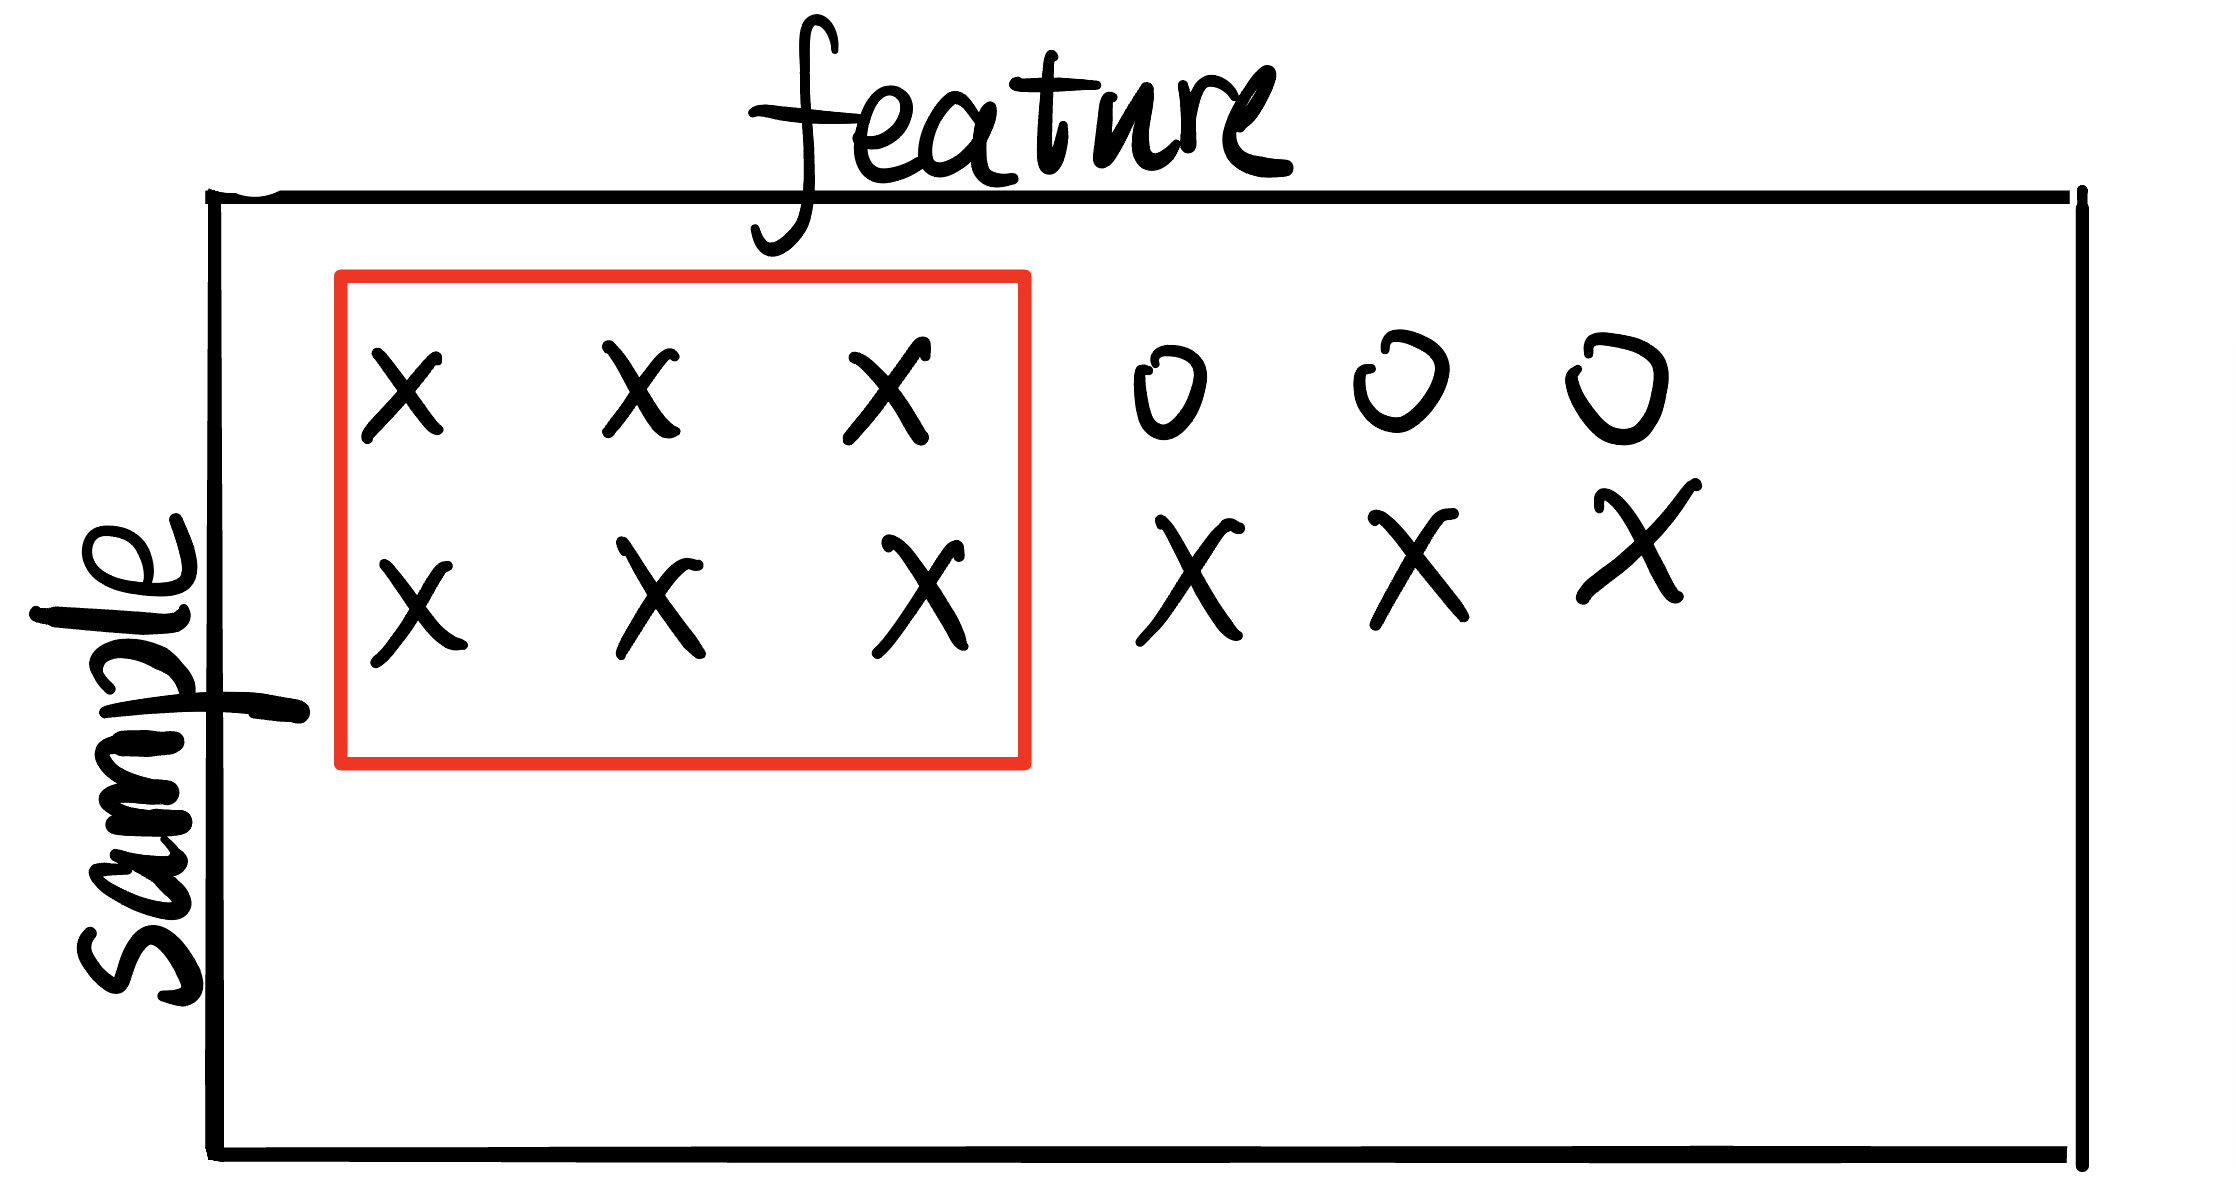
\includegraphics[width=0.6\textwidth]{idea.jpeg}
        % \caption{Idea of our method}
        % \label{fig:idea}
    \end{figure}
\end{frame}

% \begin{frame}{Contributions}
%     \begin{itemize}
%         \item \textbf{Enhanced Co-clustering:} Developed a sophisticated co-clustering technique that concurrently categorizes the rows and columns of a matrix. This approach is particularly effective for managing incomplete data, as it elucidates the similarities between samples even when attributes are missing, thereby facilitating more robust and accurate analyses.
        
%         \item \textbf{Optimized Parallelism:} Implemented an advanced parallel processing framework, enhancing computational efficiency and resource utilization. This optimization enables the method to be more adaptable and scalable to diverse computing environments and large datasets.
        
%         \item \textbf{Probabilistic Modeling:} Formulated a rigorous probabilistic model to underpin the proposed method, providing theoretical assurances regarding the reliability and validity of the obtained results. This model serves as a foundational pillar, ensuring the robustness and integrity of the analytical outcomes.
%     \end{itemize}
% \end{frame}

% Other things to mention
% 1. Tried multi ellipses but 1. though good on pure 2. not big progress on many many ellipses because the challenge with be the good detection on arcs when noise is envolved and 3. I find no application scenario.
% 2. Application on election -> NLP
% 3. Application on food nutrition and market -> Recommender systems
% So I find two possible application scenarios, one is NLP and the other is recommender systems.

\begin{frame}{Research Findings and Observations}
    \begin{itemize}
        \item \textbf{Big size simulation:} $100000\times 100000$ matrix resulting good performance.
        \item % include result.png
        \begin{figure}
            \centering
            
\includegraphics[width=0.8\textwidth]{result.png}
            % \caption{Result of $100000\times 100000$ matrix}
            % \label{fig:result}
        \end{figure}
        \item \textbf{Multi-Ellipses Expansion:} 
        \begin{itemize}
            \item Achieved $92.7\%$ accuracy on pure ellipse images.
            \item Struggled with accurate arc detection in noisy, multi-ellipse scenarios.
            \item No clear application scenario identified.
        \end{itemize}
        
        \item \textbf{Election and NLP:} 
        \begin{itemize}
            \item One research found on applying co-clustering to elections.
            \item Identified potential for clustering text and extracting themes in NLP.
        \end{itemize}
        
        \item \textbf{Food Nutrition and Market:} 
        \begin{itemize}
            \item Identified applications in recommender systems, clustering customers, and discerning preferences.
            \item Potential to provide insights into consumer behavior and preferences in food nutrition and market domains.
        \end{itemize}
    \end{itemize}
\end{frame}






\end{document}